\begin{frame}{Idea}
	\vspace{-20pt}
	\begin{figure}[htb]
		\centering
		\resizebox{\textwidth}{!}{%
			\begin{tikzpicture}
				\node at (0,0.8) {1 Geometry + 1 Force};
				\node[draw=none, inner sep=0pt] at (0,0) {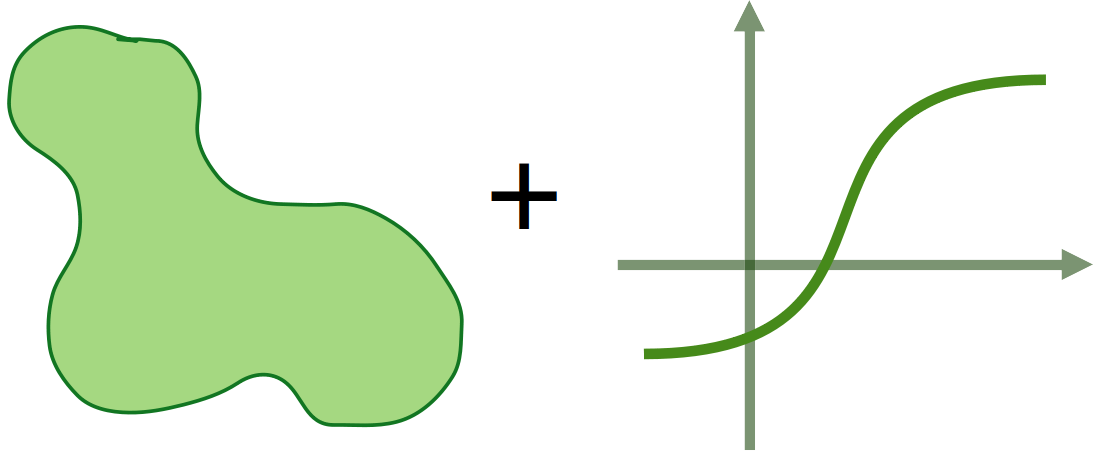
\includegraphics[width=2cm]{images/correction/objective_onegeom_onefct.png}};
				\node at (0,-1) {$\begin{aligned}[t]
						\; \phi \quad \text{\small and} \quad &f \\
						\; (\text{\small and} \quad &g)
					\end{aligned}$};
				
				\draw[->, title, line width=1.5pt] (1.7,0.1) -- (2.7,0.1);
				
				\node[align=center] at (4,1) {Get PINNs prediction};
				\node[draw=none, inner sep=0pt] at (4,0.1) {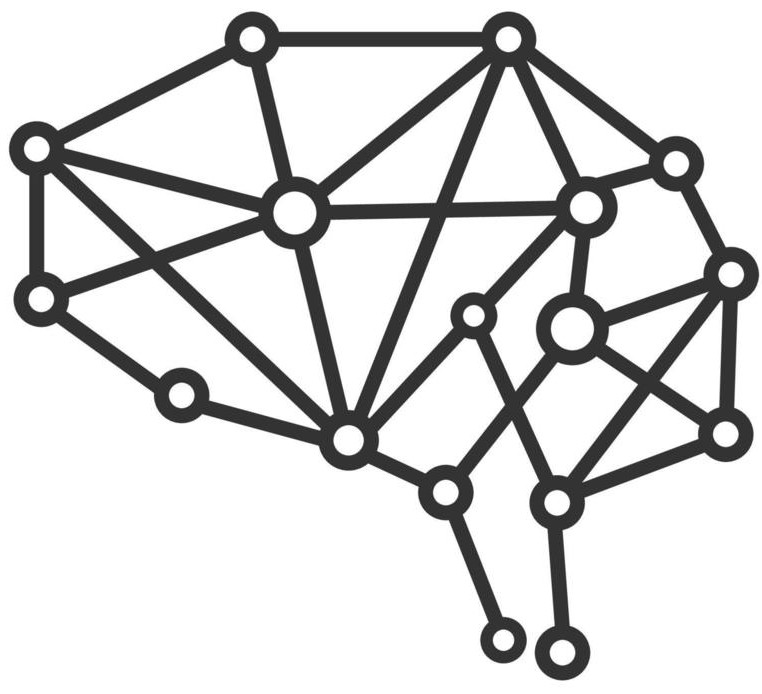
\includegraphics[width=1.4cm]{images/correction/objective_pinns.jpg}};
				\node at (4,-0.8) {\fcolorbox{blue}{white}{$u_{NN}=\phi w_{NN}+g$}};
				\node at (4,-1.3) {\textcolor{blue}{$u_{NN}=g$ on $\Gamma$}};
				
				% Ajouter une flèche entre les deux rectangles
				\draw[->, title, line width=1.5pt] (5.2,0.1) -- (6.2,0.1);
				
				\node[align=center] at (7.8,1) {Correct prediction \\ with FEM};
				\node[draw=none, inner sep=0pt] at (7.8,-0.1) {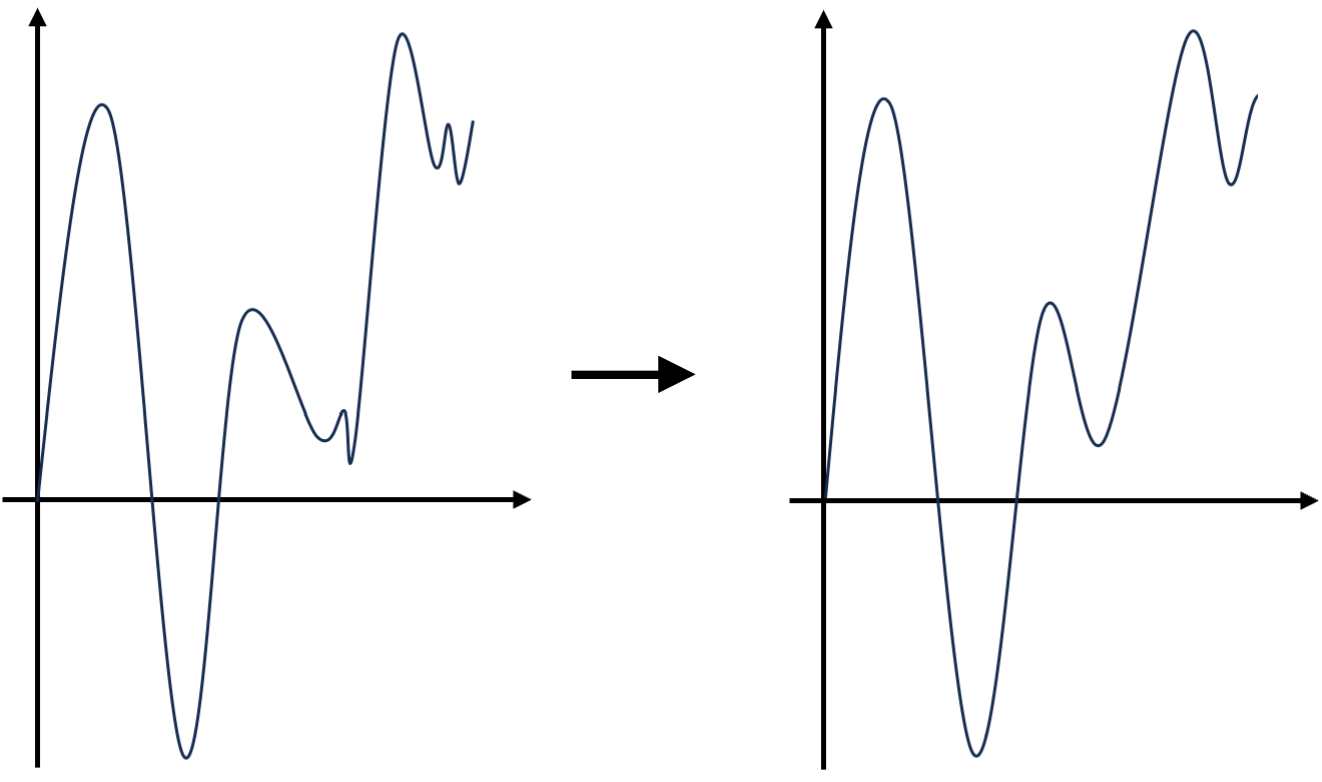
\includegraphics[width=2.5cm]{images/correction/objective_corr.png}};		
				\node at (7.8,-1) {$u_{NN}\rightarrow\tilde{u}=u_{NN}+\tilde{C}$};
			\end{tikzpicture} 
		}%
	\end{figure}
	
	\vspace{-5pt}
	
	\textbf{Correct by adding :} Considering $u_{NN}$ as the prediction of our PINNs for (\ref{edp}), the correction problem consists in writing the solution as
	\begin{equation*}
		\tilde{u}=u_{NN}+\underset{\textcolor{red}{\ll 1}}{\fcolorbox{red}{white}{$\tilde{C}$}}
	\end{equation*}
	
	\vspace{-8pt}
	\begin{minipage}{\linewidth}
		\setstretch{0.5}
		and searching $\tilde{C}: \Omega \rightarrow \mathbb{R}^d$ such that
		\begin{equation}
			\left\{\begin{aligned}
				-\Delta \tilde{C}&=\tilde{f}, \; &&\text{in } \Omega, \\
				\tilde{C}&=0, \; &&\text{on } \Gamma,
			\end{aligned}\right. \label{corr_add} \tag{$\mathcal{P}^{+}$}
		\end{equation}
		with $\tilde{f}=f+\Delta u_{NN}$. \refappendix{frame:fem} \refappendix{frame:mult}
	\end{minipage}
\end{frame}

\begin{frame}{Poisson on Square}
	Solving (\ref{edp}) with homogeneous Dirichlet BC ($g=0$). \\
	\ding{217} \textbf{Domain (fixed) :} $\Omega=[−0.5\pi,0.5\pi]^2$ \\
	\ding{217} \textbf{Analytical levelset function :}
	\small
	\begin{equation*}
		\phi(x,y)=(x-0.5\pi)(x+0.5\pi)(y-0.5\pi)(y+0.5\pi)
	\end{equation*} 
	\ding{217} \textbf{Analytical solution :}
	\small
	
	\vspace{-8pt}
	\begin{equation*}
		u_{ex}(x,y)=\exp\left(−\frac{(x-\mu_1)^2+(y-\mu_2)^2}{2}\right)\sin(2x)\sin(2y)
	\end{equation*} 
	\normalsize
	with $\mu_1,\mu_2\in[-0.5,0.5]$ (\textcolor{red}{parametric}). 
	
	\vspace{8pt}
	Taking $\mu_1=0.05,\mu_2=0.22$, the solution is given by
	\begin{minipage}{0.68\linewidth}
		\centering
		\pgfimage[width=\linewidth]{images/correction/poisson_sol.png}
	\end{minipage}
	\begin{minipage}{0.28\linewidth}
		\flushright
		\pgfimage[width=0.9\linewidth]{images/correction/poisson_loss.png}
	\end{minipage}
\end{frame}

\begin{frame}{Theoretical results}
	\vspace{-8pt}
	
	\hypersetup{
		citecolor=white,
	}
	
	\begin{mytheo}{\footnotesize\citep{ours_2024}\normalsize}{add}
		We denote $u$ the solution of (\ref{edp}) and $u_h$ the discrete solution of the correction problem (\ref{corr_add}) with $V_h$ a $\mathbb{P}_k$ Lagrange space. Thus
		\begin{equation*}
			|| u-u_h ||_0 \leq \fcolorbox{orange}{other!10!white}{$\frac{|u-u_{\theta}|_{H^{k+1}}}{|u|_{H^{k+1}}}$} \left( \frac{\gamma}{\alpha} C h^{k+1} |u|_{H^{k+1}}\right)
		\end{equation*}
		with $\alpha$ and $\gamma$ respectively the coercivity and continuity constant.
	\end{mytheo}

	\hypersetup{
		citecolor=other,
	}

	Taking $\mu_1=0.05,\mu_2=0.22$. 
	\vspace{-20pt}
	\begin{center}
		\pgfimage[width=0.5\linewidth]{images/correction/theoretical.png}
	\end{center}
	\vspace{-7pt}
	\footnotesize
	\textit{Remark :} We note $N$ the number of nodes in each direction of the square.
\end{frame}

\begin{frame}{Gains using our approach}	
	Considering a set of $n_p=50$ parameters : $\left\{(\mu_1^{(1)},\mu_2^{(1)}),\dots,(\mu_1^{(n_p)},\mu_2^{(n_p)})\right\}$.
	
	\vspace{5pt}
	
	\hspace{20pt}\begin{minipage}{0.05\linewidth}
		\footnotesize
		\rotatebox[origin=b]{90}{\textbf{Solution $\mathbb{P}_1$}} 
	\end{minipage}
	\begin{minipage}{0.8\linewidth}
		\centering
		\pgfimage[height=1.7cm]{images/correction/gains_P1.png}
	\end{minipage} 

	\vspace{5pt}

	\hspace{20pt}\begin{minipage}{0.05\linewidth}
		\footnotesize
		\rotatebox[origin=b]{90}{\textbf{Solution $\mathbb{P}_2$}} 
	\end{minipage}
	\begin{minipage}{0.8\linewidth}
		\centering
		\pgfimage[height=1.7cm]{images/correction/gains_P2.png}
	\end{minipage} 

	\vspace{5pt}

	\hspace{20pt}\begin{minipage}{0.05\linewidth}
		\footnotesize
		\rotatebox[origin=b]{90}{\textbf{Solution $\mathbb{P}_3$}} 
	\end{minipage}
	\begin{minipage}{0.8\linewidth}
		\centering
		\pgfimage[height=1.7cm]{images/correction/gains_P3.png}
	\end{minipage} 
\end{frame}

\begin{frame}{Time/Precision I}	
	Taking $\mu_1=0.05,\mu_2=0.22$.
	
	\begin{minipage}{0.48\linewidth}
		\centering
		\pgfimage[width=0.9\linewidth]{images/correction/time_error.png}
	\end{minipage}
	\begin{minipage}{0.48\linewidth}
		\centering
		\pgfimage[width=0.9\linewidth]{images/correction/time_error_tab.png}
	\end{minipage}

	\vspace{10pt}

	\textbf{Question :} Where is the \textcolor{orange}{PINNs training time} ? $\qquad t_{PINNs}\approx 240s$	 
\end{frame}

\begin{frame}{Time/Precision II}	
	Taking a \textcolor{orange}{set of $n_p$ parameters} $\left\{(\mu_1^{(1)},\mu_2^{(1)}),\dots,(\mu_1^{(n_p)},\mu_2^{(n_p)})\right\}$.
	
	The time of our approach (including the PINNs training) to solve $n_p$ problems is
	\vspace{-5pt}
	\begin{equation*}
		Tot_{Add}=t_{PINNs}+n_p t_{Add}
	\end{equation*}
	and the time of FEM is
	\begin{equation*}
		Tot_{FEM}=n_p t_{FEM}.
	\end{equation*}

	Let's suppose we want to achieve an \textcolor{orange}{error of $1e-3$}. 
	
	To solve $n_p$ problems, our method is faster than FEM (when considering network training time) if
	\begin{equation*}
		Tot_{Add}<Tot_{FEM} \quad \Rightarrow \quad n_p > \frac{t_{PINNs}}{t_{FEM}-t_{Add}}\approx 5.61\quad  \Rightarrow \quad \fcolorbox{red}{white}{$n_p=6$}
	\end{equation*}
	
	\footnotesize
	\textit{Remark:} Considering that the times are of the same order for each parameter considered.	
\end{frame}

%\begin{frame}{Tableau temps}
%	\begin{table}[h]
%		\centering
%		\begin{tabular}{ccccc}
%				\toprule[1.pt]
%				& \multicolumn{2}{c}{\textbf{N}} & \multicolumn{2}{c}{\textbf{time (s)}} \\
%				\cmidrule(lr){2-3} \cmidrule(lr){4-5}
%				\textbf{Precision} & \textbf{FEM} & \textbf{Add} & \textbf{FEM} & \textbf{Add} \\
%				\cmidrule(lr){1-1} \cmidrule(lr){2-3} \cmidrule(lr){4-5}
%				\textbf{$1e-3$} & 120 & 8 & \fcolorbox{orange}{white}{43} & \fcolorbox{red}{white}{0.24} \\
%				\textbf{$1e-4$} & 373 & 25 & 423.89 & 1.93 \\
%				\bottomrule[1.pt]
%			\end{tabular}
%	\end{table}
%
%	\vspace{-5pt}
%	\small
%	\hspace{190pt} \begin{minipage}{0.1\linewidth}
%			\textcolor{orange}{$t_{FEM}$}
%		\end{minipage} \hspace{8pt} \begin{minipage}{0.1\linewidth}
%			\textcolor{red}{$t_{Add}$}
%		\end{minipage}
%\end{frame}